\documentclass[a4paper, 11pt]{article}


\usepackage{preambule}


\begin{document}

% The title page
    \import{./}{title}
\clearpage


% The table of contents
\tableofcontents
\thispagestyle{empty}
\clearpage


\setcounter{page}{1}
% The introduction
%% The study's challenges
%%% The importance of energy and energy storage
%%% The interest, usages and challenges of SCs
%%% Describing the SCs
%% Presenting the methods and tools
%%% Presenting Molecular Dynamics and LAMMPS
%%% Describing the data extracting/processing task
%%% Enumerating the additionnal tools
%% Presenting the plan
\section*{Introduction}

    % The study's challenges
%% The importance of energy and energy storage
En 2019, la consommation mondiale d'énergie finale a doublé par rapport à 1973 et a dépassé la barre des \qty{400}{\exa \joule}, dont \qty{19.7}{\percent} d'électricité \cite{birol_key_nodate}.\\
Il est donc nécessaire de pouvoir stocker efficacement l'énergie produite, c'est-à-dire avec un minimum de pertes, une grande capacité de stockage, et des temps de charge et de décharge courts.

%% The interest, usages and challenges of SCs
Les supercondensateurs sont des systèmes de stockage d'énergie caractérisé par une haute densité de puissance. À l'inverse des condensateurs habituels, ils sont capables de stocker de plus grandes quantités d'énergie.
Bien que leurs réserves soient bien loin des batteries, ils ont l'avantage de pouvoir se charger ou se décharger bien plus rapidement.\\
Ceci explique donc leur utilisation répandue pour les véhicules électriques, systèmes d'alimentation sans fil ou encore appareils portables.\\
Enfin, malgré le nombre d'études ayant déjà été menées, le fonctionnement de ces appareils reste encore peu compris. Ainsi, nous suivons une piste sérieuse\cite{bo_design_2018} pour approfondir notre compréhension avec les simulations de Dynamique Moléculaire d'électrodes capacitives.

%% Describing the SCs
Les supercondensateurs sont composés d'électrodes poreuses séparées par une membrane perméable et plongées dans un électrolyte. Ceci permet le déplacement des charges d'une électrode à l'autre lorsque l'appareil est en charge ou en décharge (\autoref{fig:schema_supercondensateur}).

\begin{figure}[hb]
    \centering
    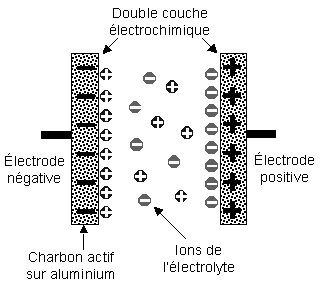
\includegraphics[height=5cm]{supercondensateur.png}
    \caption{Schéma d'un supercondensateur}
    \label{fig:schema_supercondensateur}
\end{figure}

Les électrodes capacitives sont généralement constituées de charbon actif : la porosité de telles électrodes permet d'augmenter la surface de contact avec l'électrolyte pour atteindre des capacitance spécifique de \qtyrange[range-units = single]{100}{300}{\farad \per \gram}.\\
Quant aux électrolytes, ils peuvent être groupés en fonction de leur nature : aqueux, organiques et ioniques. Parmi les électrolytes aqueux se démarquent\cite{zhong_review_2015} les électrolytes acides (\ce{H2SO4}), alkalins (\ce{KOH}), et neutres (\ce{Na2SO4}).

% Presenting the methods and tools
%% Molecular Dynamics and LAMMPS
Lors de cette étude, nous utilisons \emph{Large Atomic/Molecular Massively Parallel Simulator} (LAMMPS) pour effectuer des simulations de Dynamique Moléculaire. En effet, cet outil permet de mettre en place des simulations et d'en contrôler les conditions relativement facilement (contrôle du/des potentiel/s, de l'ensemble thermodynamique, thermostat, barostat, etc.).
%% The data extracting and processing task
Aussi, l'extraction et le traitement des données de simulations ont été une tâche non-négligeable. Pour cela, nous avons utilisé majoritairement des programmes écrits en C dont la conception et réalisation sont détaillées en annexes.\\
%% The additionnal tools
Enfin, pour des outils supplémentaires ont été utilisés pour les tâches restantes comme la visualisation des trajectoires\cite{ovito} ou encore la réalisation de configurations initiales\cite{martinez_packmol_2009}.

% Presenting the plan
La structure des électrodes capacitives étant très complexe du fait du grand nombre de pores et de leur diversité, nous avons préféré adopter un système modèle, que nous présentons en première section.\\
Puis, nous présenterons les outils que nous utilisons pour simuler un supercondensateur en charge, à savoir le potentiel réactif \emph{ReaxFF}\cite{van_duin_reaxff_2001}\cite{russo_atomistic-scale_2011}\cite{senftle_reaxff_2016} et \emph{EChemDID}\cite{onofrio_voltage_2015}.\\
Enfin, nous présentons les résultats obtenus et observations faites lors de cette étude, notamment par rapport à l'adsorption des ions à la surface des électrodes et la répartition des charges en leur sein.

\clearpage


% Presenting the model system
%% Interest of the model
%% Description
%% Simulations details
\section{Présentation du système modèle}

    % Interest of the model
Comme mentionné précédemment, à cause de la complexité du système il est préférable pour cette étude de considérer un sytème modèle. Dans cette section, nous décrivons le modèle et ses caractéristiques, avant de détailler sa construction, et de discuter des simulations dans lesquelles il intervient.

% Description
    \subsection{Description du modèle}

Le système modèle est composé d'électrodes en graphites immergées dans un électrolyte aqueux d'hydroxyde de sodium, sa structure est présentée à la \autoref{fig:schema_structure} et ses caractéristiques au \autoref{tab:caracteristiques_systeme}.

\begin{figure}[h!]
    \centering
    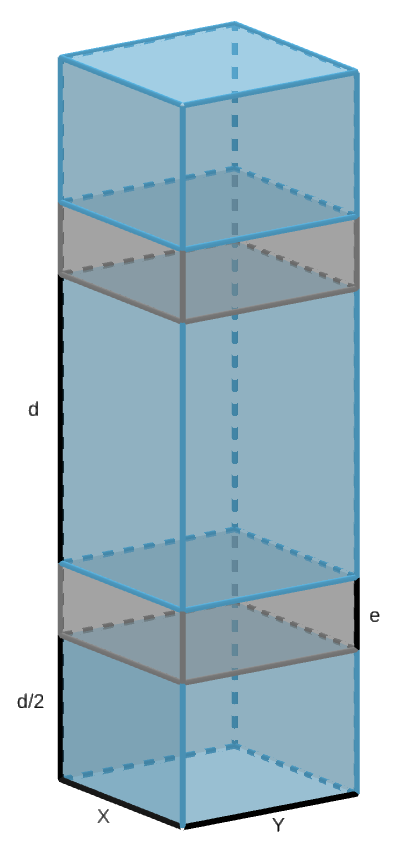
\includegraphics[height = 5 cm]{schema_structure.png}
    \caption{Schéma de la structure du système modèle}
    \label{fig:schema_structure}
\end{figure}

\begin{table}[h!]
    \centering
    \begin{tabular}{l || l | l l}
        \hline
        Groupe &Caractéristique &Valeur &\\
        \hline
        Système &Dimensions &$(22.104, 21.270, \sim 60)$ &\unit{\angstrom}\\
        &Particules &$\sim \num{3000}$ &\\
        \hline
        Électrodes &Séparation &$\sim \num{20}$ &\unit{\angstrom}\\
        &Atomes (par électrode) &\num{540} &\\
        \hline
        Électrolyte &Molécules d'eau &\num{628} &\\
        &Concentration &$\sim \num{1.0}$ &\unit{\mole \per \liter}\\
        &Ions &\num{12} &\\
        \hline
    \end{tabular}
    \caption{Caractéristiques du système}
    \label{tab:caracteristiques_systeme}
\end{table}

% Construction
    \subsection{Construction du modèle}

\begin{figure}[h!]
    \centering
    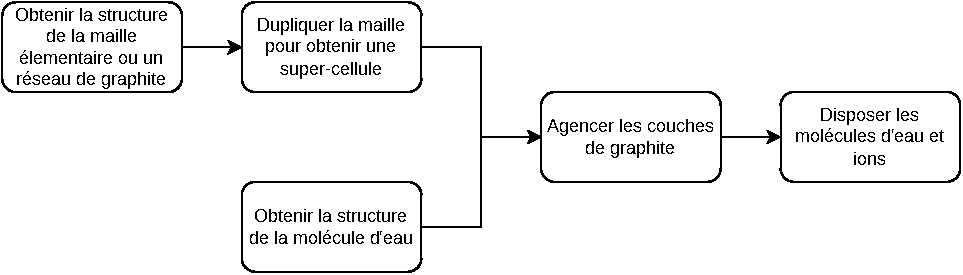
\includegraphics[height = 3 cm]{construction_structure.pdf}
    \caption{Démarche de construction de la structure}
    \label{fig:construction_structure}
\end{figure}

Pour construire la structure du modèle, la démarche \autoref{fig:construction_structure} a été adoptée afin d'obtenir le système aux dimensions et caractéristiques désirées, avec une configuration initiale des particules convenable.

\textbf{Obtention des structures}\\
Les données sur les structures des molécules ont été obtenues grâce à la \href{http://www.crystallography.net/cod/}{Crystallography Open Database} (COD) et celles-ci sont présentées à la \autoref{fig:molecules_initiales}.

\begin{figure}[h!]
	\centering
	\begin{subfigure}[t]{.49\textwidth}
		\centering
		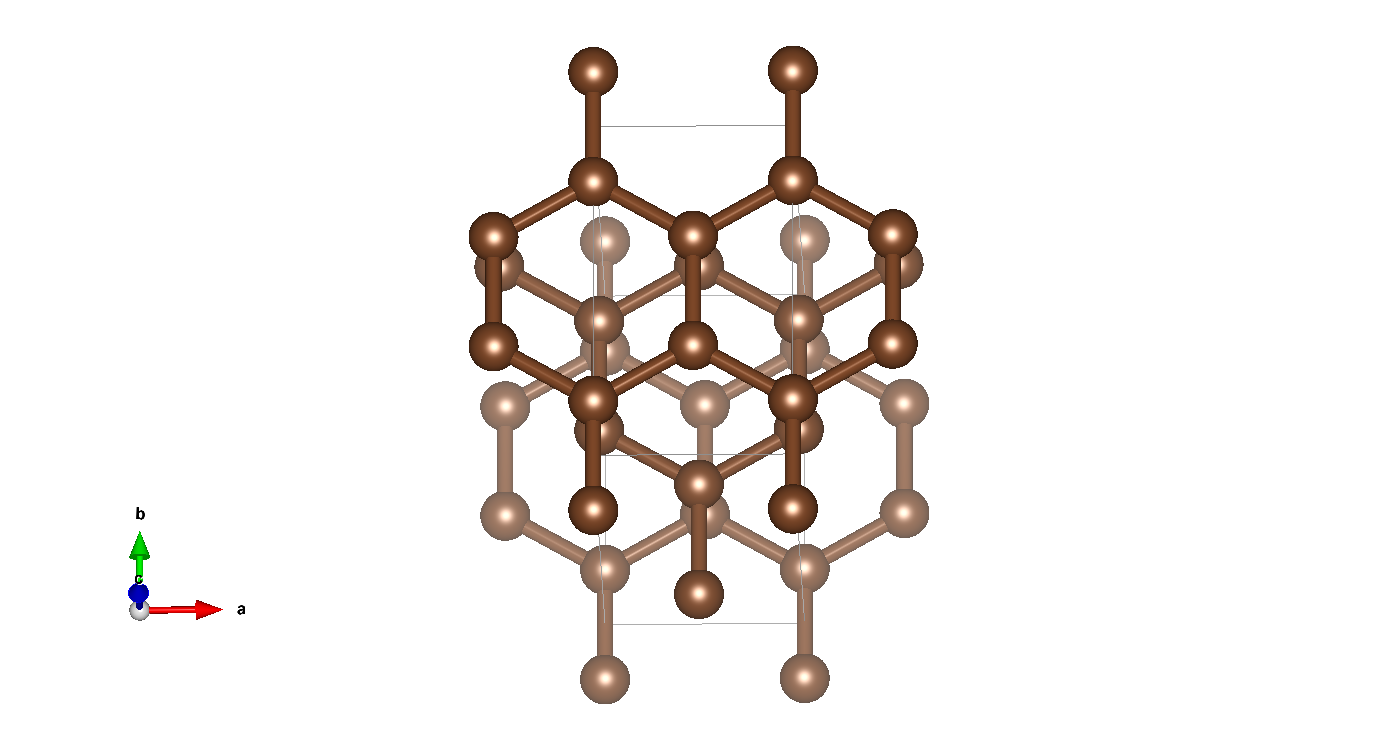
\includegraphics[width = \textwidth]{graphite.png}
		\caption{Réseau de graphite}
	\end{subfigure}%
    ~
	\begin{subfigure}[t]{.49\textwidth}
		\centering
		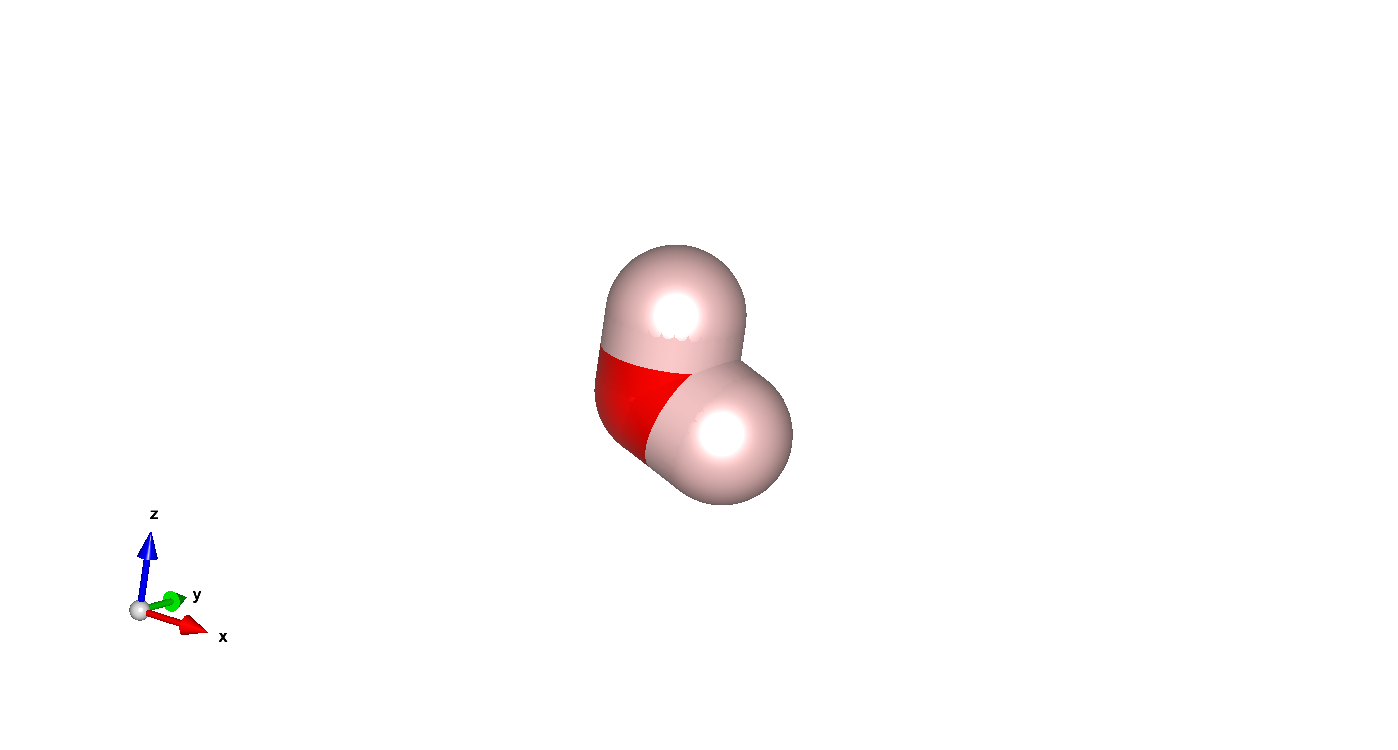
\includegraphics[width = \textwidth]{water.png}
		\caption{Molécule d'eau}
	\end{subfigure}
	\caption{Structures des molécules provenant de la COD}
	\label{fig:molecules_initiales}
\end{figure}

\textbf{Obtention de la super-cellule}\\
La structure de graphite de base a pu être étendue grâce à un logiciel tier\cite{momma_vesta_2011}, \num{9} fois selon la direction $[OX)$ et \num{5} fois selon la direction $[OY)$ afin que les dimensions dans ces directions soient du même ordre, pour obtenir une électrode de graphite (\autoref{tab:dimensions_structures} et \autoref{fig:electrode}).

\begin{table}[h!]
    \centering
    \begin{tabular}{l | c c c}
        \hline
        Structure &X [Å] &Y [Å] &Z [Å]\\
        \hline
        Réseau initial &\num{2.456} &\num{4.254} &\num{6.696}\\
        Électrode de graphite &\num{22.104} &\num{21.270} &\num{6.696}\\
        \hline
    \end{tabular}
    \caption{Dimensions des sctructures}
    \label{tab:dimensions_structures}
\end{table}

\begin{figure}[h!]
    \centering
    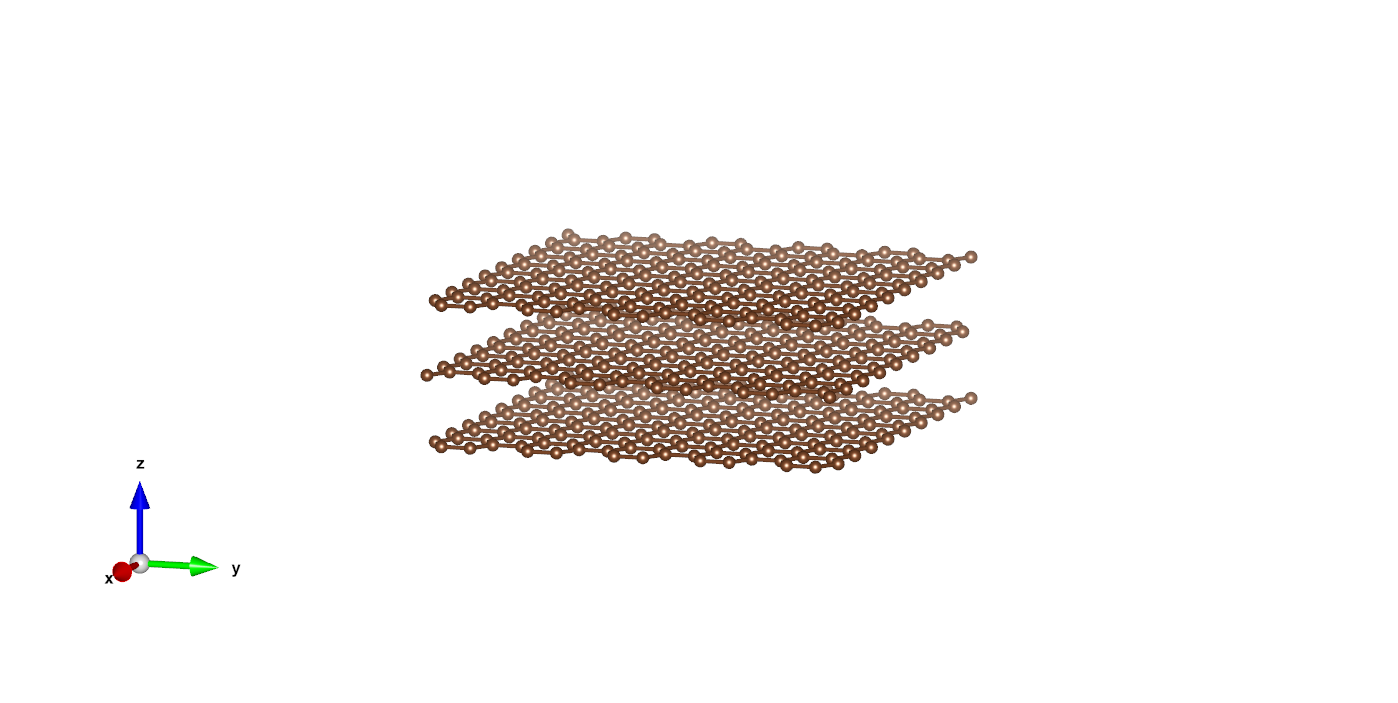
\includegraphics[height = 5 cm]{electrode.png}
    \caption{Électrode obtenue après duplication du réseau de graphite : {\footnotesize les couches de graphènes sont séparées d'environ $\sim$\qty{3.5}{\angstrom}.}}
    \label{fig:electrode}
\end{figure}

\textbf{Agencement des particules}\\
Les particules ont pu être disposées pour construire le modèle à l'aide de \packmol{}\cite{martinez_packmol_2009}, détails à l'\autoref{apdx:packmol}.

Pour obtenir des configurations initiales suffisamment stables nous avons choisi de répartir les entités en les séparant d'au moins \qty{2.5}{\angstrom} : entre les molécules et ions de l'électrolyte, et entre les particules de l'électrolyte et les électrodes.\\
Et pour respecter les conditions aux limites périodiques, cette séparation a également été appliquée aux bords du système : nous ajoutons un retrait égal à la moitité de cette séparation à chaque bord.

Finalement, nous obtenons la configuration présentée à la figure \autoref{fig:structure_finale}.

\begin{figure}[h!]
    \centering
    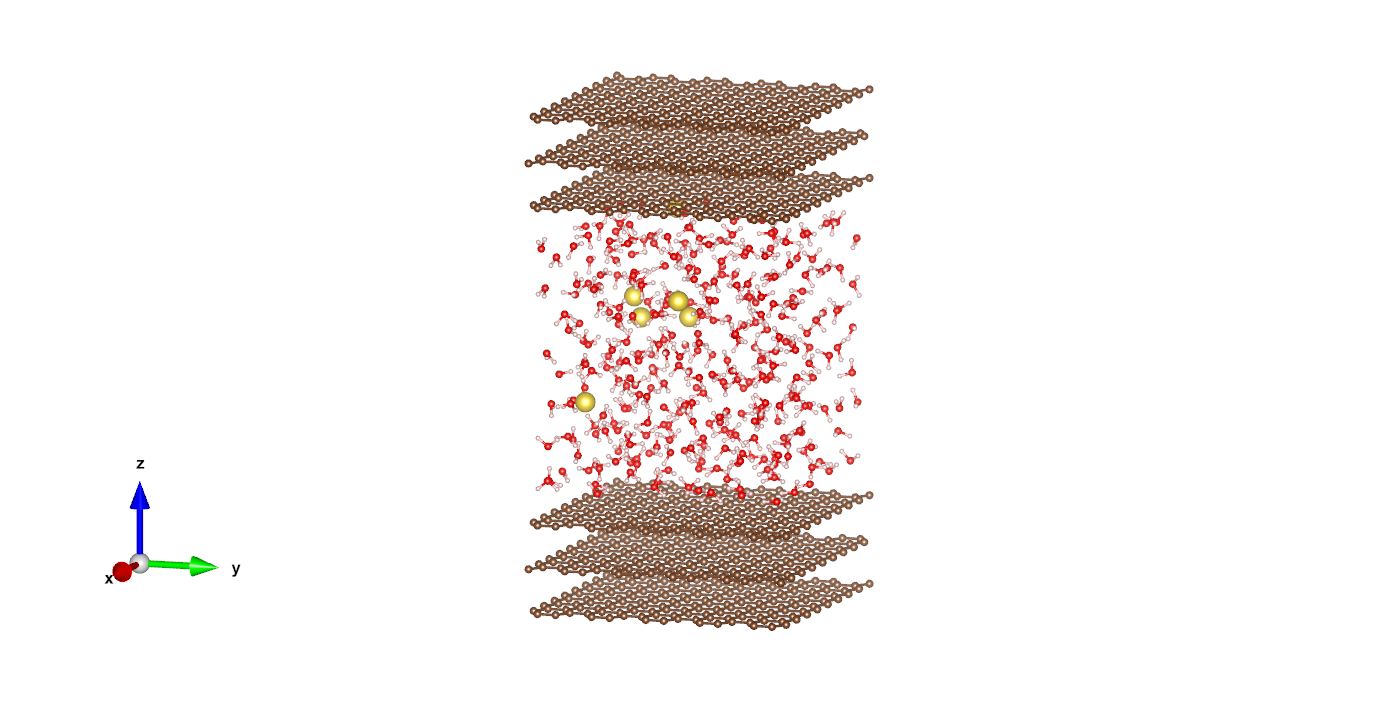
\includegraphics[height = 5 cm]{structure.png}
    \caption{Structure finale obtenue après agencement des molécules}
    \label{fig:structure_finale}
\end{figure}

% Simulations details
    \subsection{Déroulement et détails des simulations} \label{sec:deroulement_simulations}

\begin{table}[h!]
    \centering
    \begin{tabular}{l || l | l l}
        \hline
        Étape &Paramètre &Valeur &\\
        \hline
        Toutes &\lstinline!timestep! &\num{0.1} &\unit{\femto \second}\\
        &potentiel &\reaxff{} &\\
        \hline
        Minimisation &\lstinline!maxiter! &\num{1000} &\\
        &\lstinline!maxeval! &\num{10000} &\\
        &\lstinline!etol! &\num{e-05} &\\
        &\lstinline!ftol! &\num{e-06} &\unit{\kilo \cal \per \mole \per \angstrom}\\
        \hline
        Relaxation et Stabilisation &durée &\num{200000} &\\
        & &\num{20.0} &\unit{\pico \second}\\
        &\lstinline!T_target! &\num{300.0} &\unit{\kelvin}\\
        &\lstinline!P_target! &\num{1.0} &\unit{\atm}\\
        \hline
        Simulation &durée &\num{10000000}\\
        &polarisation &\echemdid{} &\\
        & &\num{1.0} &\unit{\nano \second}\\
        &\lstinline!T_target! &\num{300.0} &\unit{\kelvin}\\
        \hline
    \end{tabular}
    \caption{Récapitulatif des paramètres des simulations}
\end{table}

\begin{figure}[h!]
    \centering
    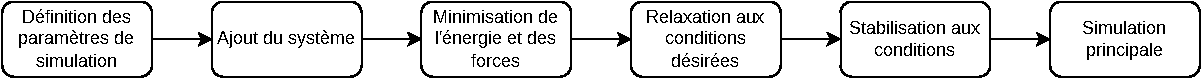
\includegraphics[width = \textwidth]{deroulement_simulations.pdf}
    \caption{Déroulement des simulations}
    \label{fig:deroulement_simulations}
\end{figure}

Toutes les simulations suivent le déroulement de la \autoref{fig:deroulement_simulations} afin de définir les paramètres de simulation, de préparer le système, et de lui permettre de s'équilibrer.

\textbf{Paramétrisation}\\
Elle consiste à définir les paramètres clés de la simulation. Par exemple :
\begin{itemize}
    \item le pas de temps (\lstinline!timestep!) sélectionné pour les simulations est de \qty{0.1}{\femto \second}
    \item les interactions sont basés sur le potentiel réactif \reaxff{} (détaillé à la \autoref{sec:reaxff})
    \item la mise en place de la différence de potentiel entre les électrodes est réalisée grâce à \echemdid{} (détaillé à la \autoref{sec:echemdid})
\end{itemize}

\textbf{Ajout du système}\\
Ceci est effectué avec une commande \lammps{} de lecture de données. Pour ce faire, il est nécessaire de convertir les données des positions des particules du système (détails à la \autoref{sec:systeme_modele}) en données \lammps{} (détails à l'\autoref{apdx:conversion_lammps}).

\textbf{Minimisation}\\
Cette étape est essentielle au démarrage d'une simulation : elle sert à s'assurer que la configuration de départ de la simulation soit "correcte" et que le système soit stable.

Elle consiste à déplacer les particules du système sans dynamique de manière à minimiser l'énergie potentielle et les forces totales du système. Cette procédure suit un algorithme de gradient conjugué avec pour fonction objectif l'énergie potentielle totale :
\begin{equation*}
    E(r_1, \dots, r_N) = \sum_{i, j} E_{pair} (r_i, r_j) + \dots + \sum_{i, j} E_{fix} (r_i)
\end{equation*}
où sont prises en compte les énergies :
\begin{itemize}
    \item des interactions de paires
    \item des liaisons et angles si présents
    \item des interactions \textit{improper} ou \textit{dihedral} : les interactions mettant en jeu \num{3} ou \num{4} atomes
    \item des \lstinline!fix! imposés lors de la minimisation : des commandes \lammps{} visant à imposer des contraintes lors de la minimisation, par exemple la relaxation de la boîte pour atteindre une pression désirée, ou encore les forces désactivées pour un groupe d'atomes pour qu'ils ne subissent pas de modifications
\end{itemize}

\textbf{Relaxation et stabilisation}\\
Ces étapes utilisent un thermostat et barostat de Nosé--Hoover pour atteindre les conditions physiques recherchées et les stabiliser.

Les conditions de pression et de température recherchées sont $T = \qty{300}{\kelvin}$ et $P = \qty{1}{\atm}$, et les évolutions des quantités thermodynamiques lors de ces étapes sont typiquement celles des \autoref{fig:allures_thermostat_barostat}.

\begin{figure}[h]
    \centering
    \begin{subfigure}[t]{.49\textwidth}
        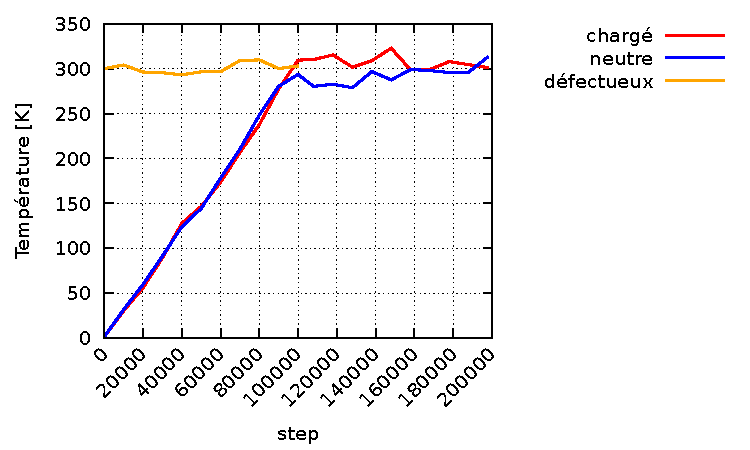
\includegraphics[width = \textwidth, draft]{relaxation_temp.pdf}
        \caption{Température}
    \end{subfigure}%
    ~
    \begin{subfigure}[t]{.49\textwidth}
        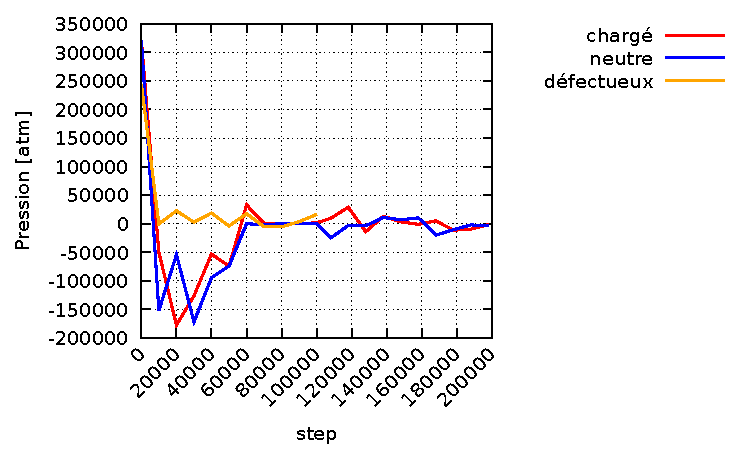
\includegraphics[width = \textwidth, draft]{relaxation_press.pdf}
        \caption{Pression}
    \end{subfigure}
    \begin{subfigure}[t]{.49\textwidth}
        \includegraphics[width = \textwidth, draft]{relaxation_density.pdf}
        \caption{Densité}
    \end{subfigure}
    \caption{Allures des grandeurs thermodynamiques pendant de la relaxation et la stabilisation {\tiny (chaque étape a lieu en \num{100000} \lstinline!timestep!s soit \qty{10}{\pico \second})}}
    \label{fig:allures_thermostat_barostat}
\end{figure}

\textbf{Simulation}\\
Cette étape sert à récolter des données et informations sur le système après qu'il a atteint l'équilibre.

Elle se déroule avec un thermostat de Nosé--Hoover à \qty{300}{\kelvin} et pour une durée $\geq~\qty{1}{\nano \second}$ (\autoref{fig:allures_simulation_principale}).

\begin{figure}[h]
    \centering
    \begin{subfigure}[t]{.49\textwidth}
        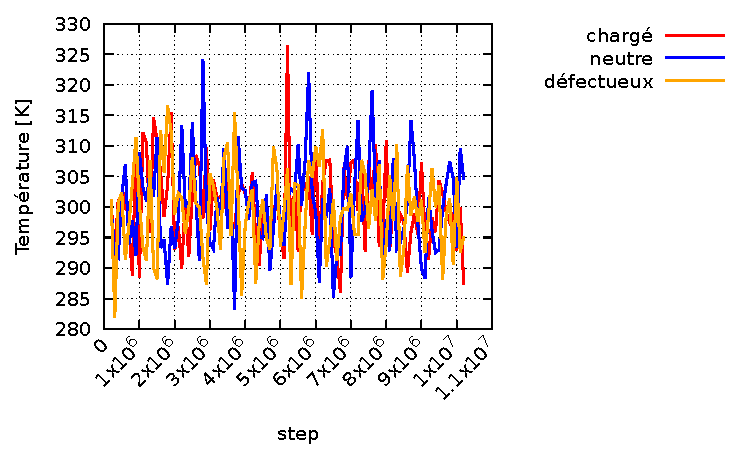
\includegraphics[width = \textwidth, draft]{main_temp.pdf}
        \caption{Température}
    \end{subfigure}%
    ~
    \begin{subfigure}[t]{.49\textwidth}
        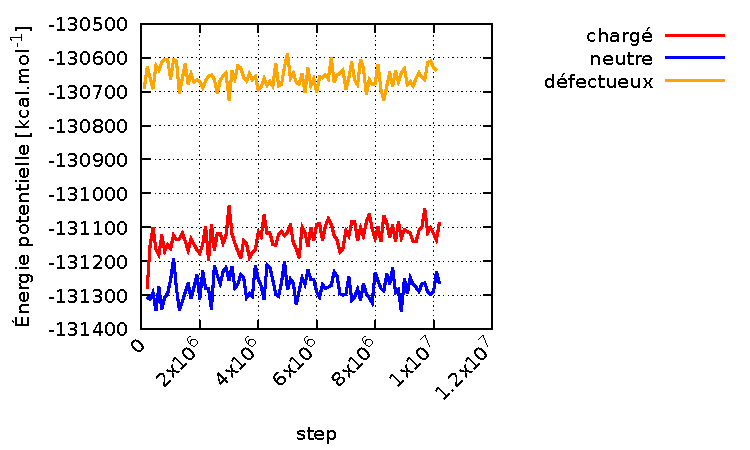
\includegraphics[width = \textwidth, draft]{main_epot.pdf}
        \caption{Énergie potentielle}
    \end{subfigure}
    \begin{subfigure}[t]{.49\textwidth}
        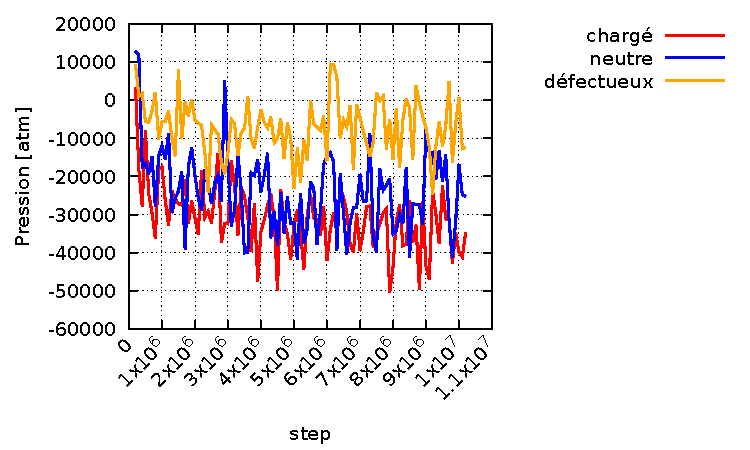
\includegraphics[width = \textwidth, draft]{main_press.pdf}
        \caption{Pression}
    \end{subfigure}
    \caption{Allures des grandeurs thermodynamiques pendant la simulation principale}
    \label{fig:allures_simulation_principale}
\end{figure}


% Presenting the materials and methods
%% Presenting ReaxFF
%%% Theoretical
%%% The LAMMPS implementation
%% Presenting EChemDID
%%% Presenting CC, CV and Qeq
%%% Presenting EChemDID
\section{Présentation des méthodes utilisées}


% Presenting the results
%% Comparing two water models
%% Charge distribution
%% Ions adsorption/displacement
\section{Résultats et discussion}


% Conclusion
\section{Conclusion}


% References
\printbibliography

\end{document}